\section{Feature Representation Learning}
\label{feature-learning:sec}

In this step, \tool aims to learn the node feature embeddings based on the node features generated from step 1. So the input of this step is the method-level and statement-level graphs, and the expected output is the node embedding vectors for each node in each graph.

To be more detailed, we also introduce the node feature representation learning from both method-level and statement-level.

\subsection{Method-level Feature Representation Learning}

\begin{figure}[t]
	\centering
	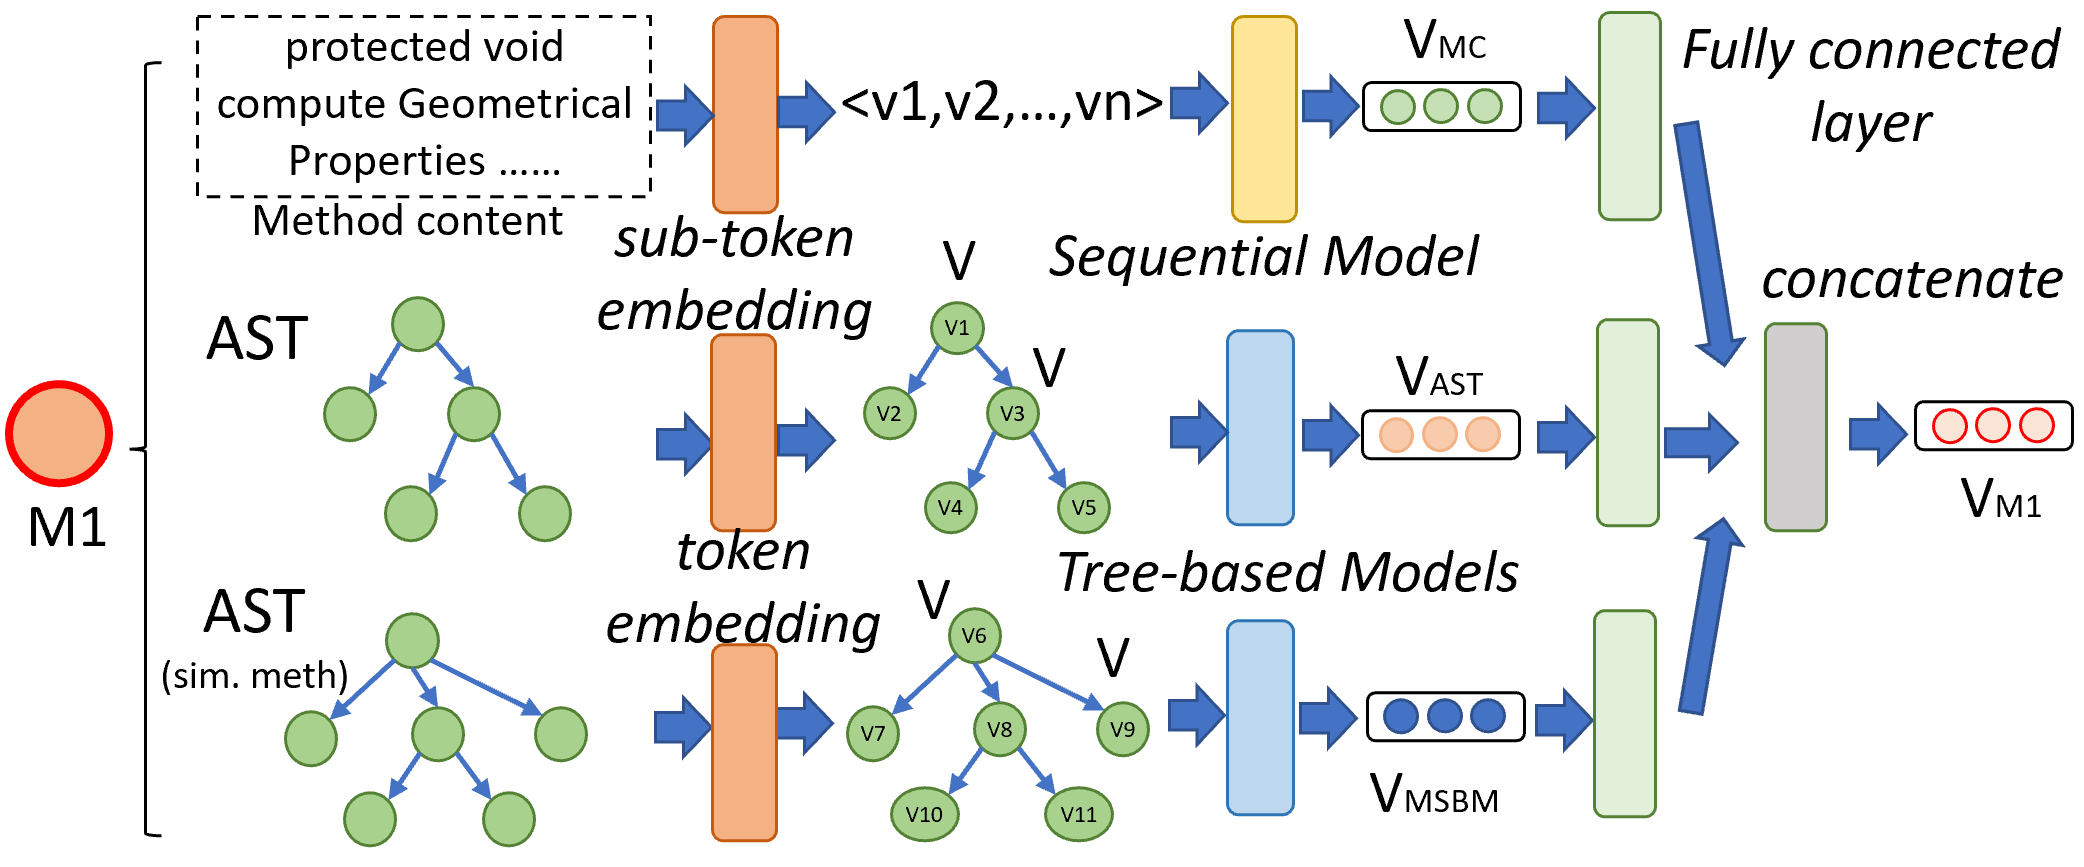
\includegraphics[width=3.4in]{graphs/step-2-method-new.png}
	\caption{Method-level Feature Representation Learning}
	\label{method-level-feature-learning}
\end{figure}

From step 1, for each node representing a method $M$, there are extracted sequences of sub-tokens $Seq^p_m$ as the method content, generated AST $Tree_m$, and the generated AST for the most similar buggy method $M_b$ as the node features. Thus, to learn the feature representation, we follow these steps.

1) {\em \underline{The method's content}}: \tool uses the token embedding techniques to learn the representation vector for each token in the sequence and then replace each sub-token with the embedding vector generated from the techniques. The GloVe \cite{pennington2014glove} is a good word embedding technique that can catch the meaning of the sub-token well, so \tool uses GloVe as the token embedding technique. After the vectorization, \tool has a sequence of vector $Seq^{pe}_m$ and then uses a sequential model to learn the summarized vector that can represent the method's content.  GRU layer \cite{cho2014learning} is a type of RNN layer that is efficient in learning and summarizing the information in the sequences. \tool uses the GRU layer here to learn the embedding vector $V_{mc}$ for the method content. For example, as you can see in Figure \ref{method-level-feature-learning}, the method content first goes through the sub-token embedding bar and become a sequence of vectors. Each vector inside represents a sub-token. Such as $V_{geometrical}$ represent the sub-token $geometrical$. And then, this sequence is feed into the sequential model and gets the $V_{mc}$ as a summary to represent the method content.

2) {\em \underline{The method's structure}}: Similarly, \tool firstly uses the GloVe to vectorize the AST just as in 1) and then uses a tree-based model to learn the method's structure. One of the most recent studies, TreeCaps \cite{bui2021treecaps} proves that it is good at learning the tree structure information. So \tool uses TreeCaps as the tree-based model to learn the embedding vector $V_{AST}$ to catch the tree structure information. As shown in Figure \ref{method-level-feature-learning}, the generated AST firstly has been vectorized with GloVe and then use the tree-based model to get the representation vector $V_{AST}$

3) {\em \underline{Most similar buggy method}}: As for the similar buggy method, \tool doing the same process as the method structure feature by using the GloVe and TreeCaps to learn the embedding vector $V_{MSBM}$. Similar as feature 2), in figure \ref{method-level-feature-learning}, the bottom line shows how the vector $V_{MSBM}$ generated for method $M1$

\subsection{Statement-level Feature Representation Learning}

\begin{figure}[t]
	\centering
	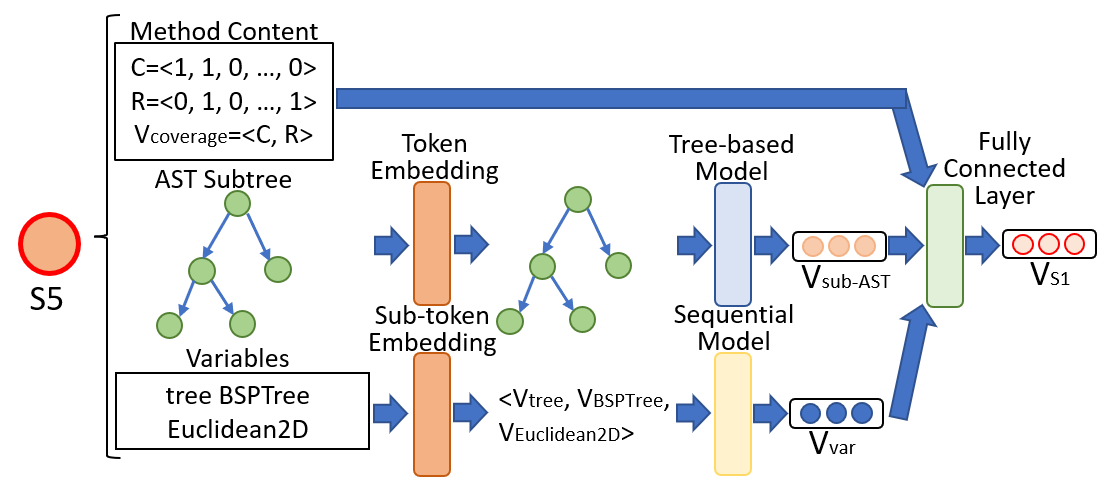
\includegraphics[width=3.4in]{graphs/step-2-statement-new.png}
	\caption{Statement-level Feature Representation Learning}
	\label{statement-level-feature-learning}
\end{figure}

From step 1, for each node representing a statement $S$, there are extracted code coverage information vector, generated AST subtree $Tree_s$, and the generated variable sequence as the node features. Thus, to learn the feature representation, we follow these steps.

1) {\em \underline{Code Coverage}}: \tool does not make any changes and directly regard $V_{Cov} = <c_1, c_2, ...,
c_K, r_1, r_2, ..., r_K>$ that is extracted from step 1 as the embedding vector $V_{cc}$ for the code coverage. 

2) {\em \underline{The statement's structure}}: \tool does the same process as the method's structure feature. \tool firstly using the GloVe to vectorize the AST and then using tree-based model TreeCaps to learn the embedding vector $V^{subtree}$. Just like the process steps for the AST subtree feature in Figure \ref{statement-level-feature-learning}.

3) {\em \underline{List of variables}}: As for the similar buggy method, \tool doing the same process as the method structure feature by using the GloVe and TreeCaps to learn the embedding vector $V^{var}$. For example, in Figure \ref{statement-level-feature-learning}, the variable sequence $tree BSPTree Euclidean2D$ in $S5$ has been embedded through the sub-token embedding technique into $<V_{tree}, V_{BSPTree}, V_{Euclidean2D}>$ and then the sequential model learns the representation vector $V_{var}$ for the variable sequence. 

After having the six embedding vectors mentioned above, \tool uses six fully connected layers to standardize each embedding vector's length to $l/3$ (Here l/3 is an integer). And then, for both method-level and statement-level, \tool concatenate three feature embedding vector into one vector $V_{M}$ or $V_{S}$ for the method-level or statement-level with the length of $l$. In this case, for both method-level and statement-level, \tool all has the graph $G_m$ or $G_s$ with the node embedding vector $V_{m}$ or $V_{s}$. It is the input for the next step.
